\section{Methoden}

Zu Lösung der Aufgabenstellung wird eine modifizierte Version der sogenannten YOLO (\textit{You Only Look Once}) Netzstruktur in Python unter Nutzung der Keras API implementiert. YOLO Netze zeichnen sich durch gute Detektionsergebnisse bei einer sehr hohen Trainings- und Klassifikationsperfomanz aus. So ist mithilfe des YOLO-Modells sogar auf vergleichsweise kostengünstiger Hardware eine Echtzeitschätzung der Bounding-Boxen von Objekten möglich \cite{Redmon2016}. 

\subsection{Lossberechnung und Intersection over Union}
\label{Loss_ber}
Rezatofighi1 beschreibt die \textit{Intersection over Union} (IOU) als eine performante und präzise Möglichkeit den Loss bei der Objekterkennung zu bestimmen (s. Kap 2.2). Dabei wird die IOU aus dem Quotienten der sich überlappenden Fläche \textit{(Intersection / Overlap)} und der gemeinsam gebildeten Fläche (\textit{Union}) zweier Regionen berechnet: 
\begin{equation}\label{iou}
	IOU(y_{target},y_{pred})=\frac{y_{target} \cap y_{pred}}{y_{target} \cup y_{pred}}
\end{equation}
$y_{pred}$ steht hierbei für die geschätzte und $y_{target}$ für die reale Bounding-Box der Objekte. Die graphische Interpretation der Berechnung wird in Abbildung \ref{ioubild} deutlich. Zur Berechnung der jeweiligen Flächen wird der von Rezatofighil in \cite{Rezatofighi1902} beschriebene Algorithmus implementiert. Dort ist zusätzlich eine hier nicht genutzte Erweiterung zur \textit{Generalized-IOU} beschrieben.
\begin{figure}[!h]
  \centering
  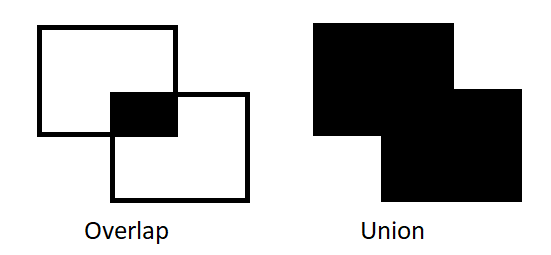
\includegraphics[width=8cm]{iou.png}
  \caption{Intersection over Union}
  \label{ioubild}
\end{figure} 
\FloatBarrier
Somit ergibt sich für den 2D-Fall als resultierende Loss-Funktion:
\begin{equation}\label{iouloss}
	L_{2D}= 1-IOU(y_{target},y_{pred})
\end{equation} 
Es ist darauf hinzuweisen, dass aufgrund der hohen Komplexität auf die Erweiterung der IOU Berechung für den 3D-Fall im Rahmen dieser Arbeit verzichtet wird. Möglich Ansätze für 3D-IOU Berechungen finden sich jedoch in \cite{Xu2019} und \cite{Mousavian1612}. Im 3D-Fall wird der Loss lediglich über den in Kapitel 2.2. beschriebenen L2-Ansatz bestimmt. In Abbildung \ref{L2_loss_graphik} ist schematisch dargestellt wie der L2 Loss berechnet wird. Hierfür wird lediglich der Abstand zwischen einem, vom Netz prädizierten Punkt und einem Zielpunkt berechnet. Dieser Abstand etspricht dem Ausdruck $y_{target}-y_{pred}$ aus Formel \ref{mse}. 
\begin{figure}[!htb]
  \centering
  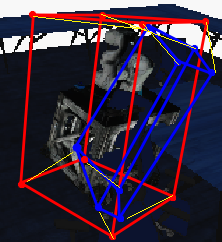
\includegraphics[width=6.2cm]{Abb/l2_loss_bei3d_bb.png}
  \caption{Prädizierte und gelabelte Punkte der Bounding-Box mit Prädiktonsfehler (Gelbe Linien)}
  \label{L2_loss_graphik}
\end{figure} 
\newpage
\subsection{Netzstruktur}

\begin{figure}[!htb]
  \centering
  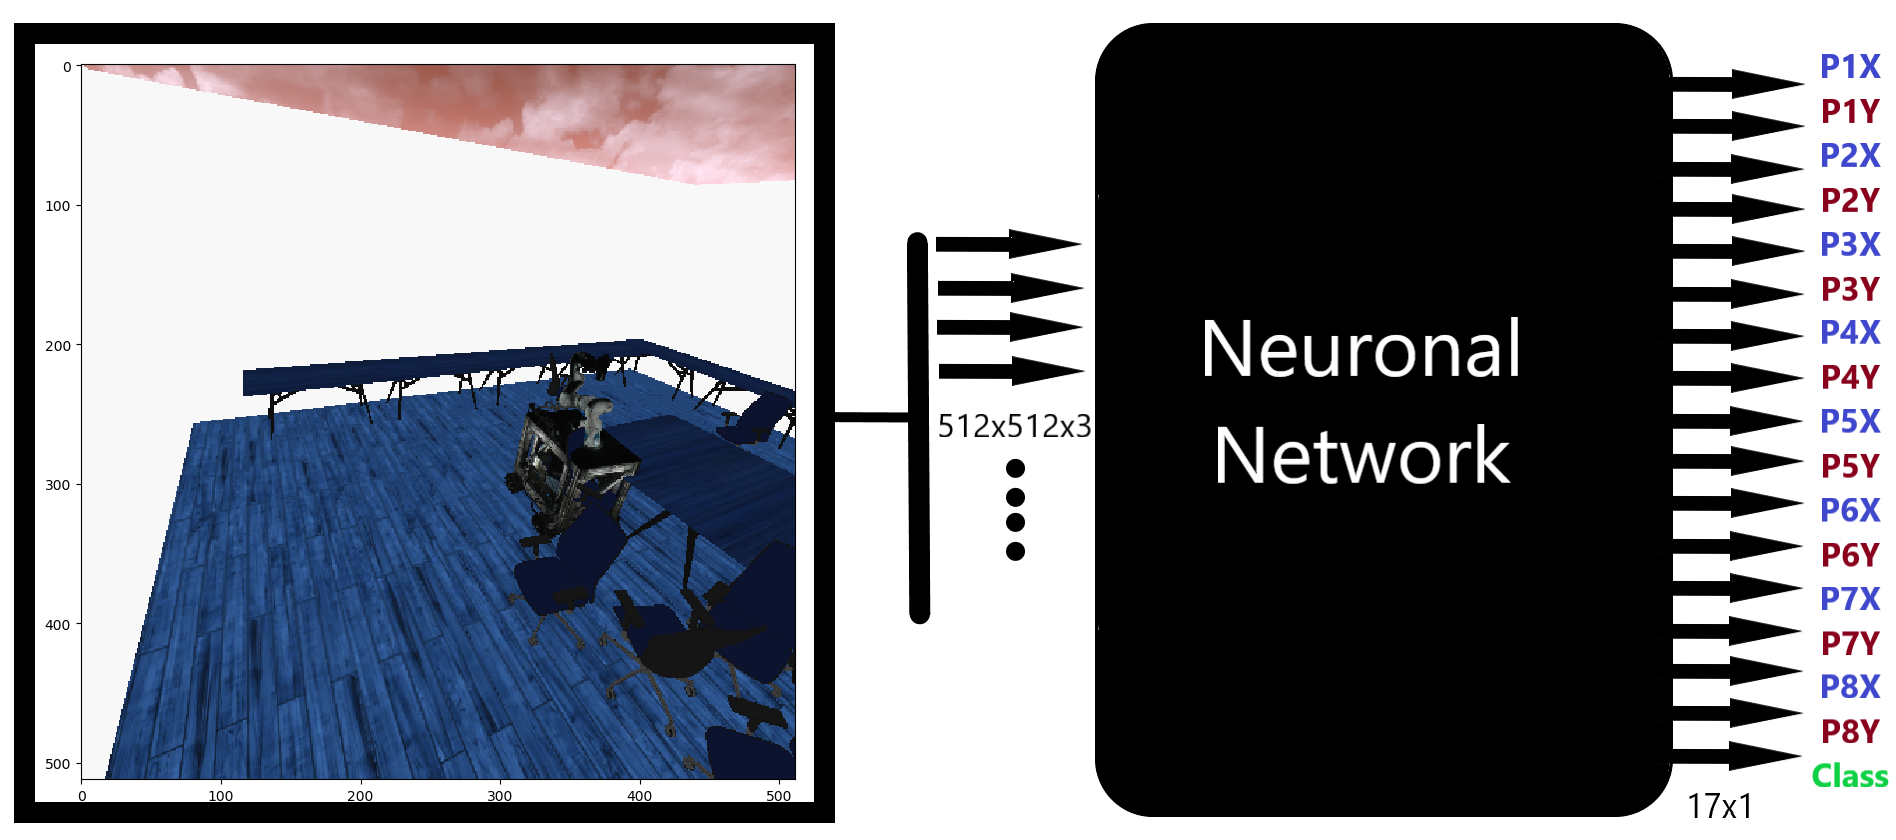
\includegraphics[width=13.8cm]{Abb/Modell_struktur.png}
  \caption{Vereinfachte Darstellung der Netzstruktur zur Prädiktion einer 3D-Bounding-Box}
  \label{grobe_netz_struktur}
\end{figure} 

Die Netzstruktur, welche für die Prädiktion einer 3D-Bounding-Box verwendet wird orientiert sich sehr stark an dem sogenannten YOLO Netz. Die ersten Schichten des Netzes bestehen aus \textit{Convolutional Layern}, welche die Aufgabe haben, Features aus dem Bild zu extrahieren. Die hintere Schicht des Netzes besteht aus  \textit{Fully Connected Layern}, welche die Koordinaten der Bounding-Box Punkte sowie die Klassenzugehörigkeit  ausgeben \cite{Redmon2016}. \\Die YOLO Netzarchitektur muss jedoch für die Prädiktion einer projizierten 3D Bounding-Box angepasst werden. Diese besitzt im Gegensatz zu einer 2D-Bounding-Box 8 anstatt 2 erforderlichen X/Y-Bildpunkten. Ein Vergleich einer 2D und einer 3D-Bounding-Box ist in Abbildung \ref{3D_Bounding_roboter} dargestellt. Aus den 8 Punkten ergeben sich 16 Koordinaten. Zu den 16 Koordinaten kommt ein weiterer Parameter, welcher die Klasse eines Objektes angibt. Diese Angabe wird implementiert, um das Netz modular und skalierbar zu halten, ist jedoch für die Lösung dieser Problemstellung nicht zwingend notwendig, da es nur die eine Klasse \textit{Roboter} gibt. In Abbildung \ref{grobe_netz_struktur} ist eine vereinfachte Darstellung des implementierten Netzes als Blackbox aufgezeigt. Zu sehen sind die 17 Ausgänge, welche aus 16 Koordinaten für die Punkte der 3D-Bounding-Box, sowie der Klassenzugehörigkeit bestehen.

\begin{figure}[!htb]
  \centering
  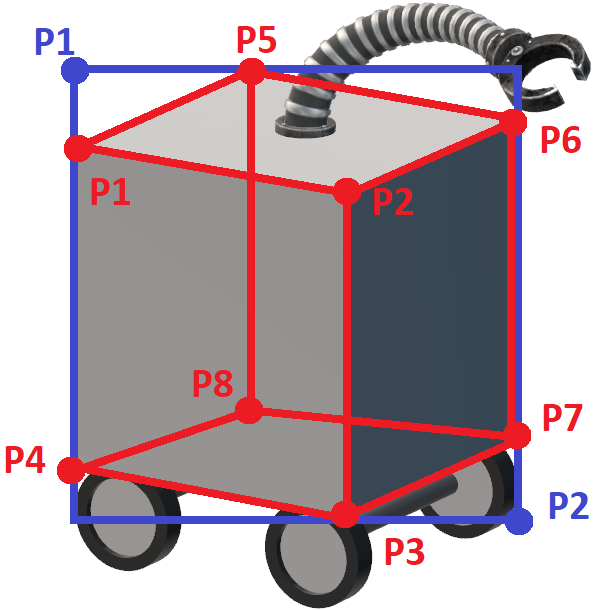
\includegraphics[width=6.8cm]{Abb/3d_robotter_mit_boundig_box_2d_vs_3d.PNG}
  \caption{3D-Bounding-Box mit 8 Punkten \textcolor{red}{(rot)} und im Vergleich dazu eine 2D-Bounding-Box mit 2 Punkten \textcolor{blue}{(blau)} }
  \label{3D_Bounding_roboter}
\end{figure} 

\newpage
\subsection{Training}
Für das Training wird ein synthetischer vorgelabelter Datensatz verwendet, welcher vom Institut für eingebettete Systeme und Medizintechnik der Hochschule Mannheim bereitgestellt wird. Es liegen insgesamt 2000 gelabelte Samples vor, von denen 90\% für das Training und 10\% für die Validierung verwendet werden. Alle weiteren Trainingsparameter sind Tabelle \ref{trainings_param} zu entnehmen. Diese optimalen Hyperparameter wurden dabei in mehreren Trainingsexperimenten empirisch ermittelt.\\

\begin{table}[!htb]

\centering
\caption{Trainingsparameter}
\begin{tabular}{ll}
\label{trainings_param}
\textbf{Parameters}                  & \textbf{Values} \\ \hline
\\Convolutional Layer        & 9      \\
Fully connected Layer       & 2      \\
Anzahl der Trainingssamples & 1800    \\
Epochen                  & 10     \\
Batch Size                  & 1     \\
Optimizer                   & Adam   \\
Learning Rate               & 0,0001 \\
Loss Function               & MSE (siehe \ref{Loss_ber})   
\end{tabular}
\end{table}
Auf einer NVIDIA GTX960M Grafikkarte mit einer \textit{NVIDIA Compute Capability} von 5, dauert das Training des Netzwerks mit den in Tabelle \ref{trainings_param} beschriebenen Parametern lediglich 25 Minuten. Diese relativ geringe Trainingszeit ist auf die hohe Performanz der YOLO Netzstruktur zurückzuführen.   
\subsection{Beschreibung der Softwaremodule}
Für die Realisierung eines Netzwerkes zur 3D-Bounding-Box-Schätzung werden mehrere Softwaremodule implementiert und Im Folgenden beschrieben. 
\subsubsection{Laden der Daten}
Das Laden der Trainingsdaten wird durch eine eigens dafür entwickelte Klasse realisiert. Die Bilder liegen im .png Format und die Labels im .json Format vor. Die Klasse lädt diese Daten, teilt diese in Trainings- und Testdaten auf und gibt die Daten als \textit{numpy arrays} zurück, sodass diese direkt für das Training verwendet werden können. In Abbildung \ref{UML_load} ist das zu der Klasse gehörige UML Diagramm mit allen Methoden dargestellt.
\begin{figure}[!htb]
  \centering
  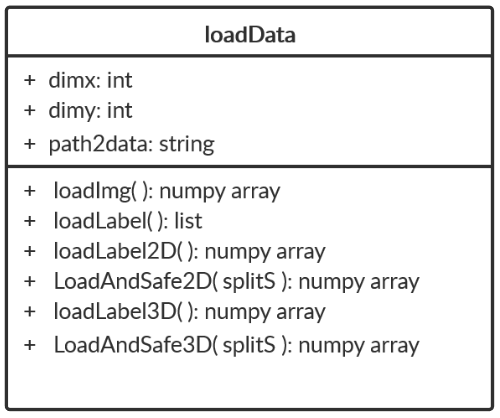
\includegraphics[width=7.8cm]{Abb/ULM_class_loadData.PNG}
  \caption{UML Diagramm loadData}
  \label{UML_load}
\end{figure} 
\subsubsection{Objekt Lokalisierung}
In der Klasse \textit{ObjectLocalizer3D} befindet sich der für die Objekterkennung und Bounding-Box-Schätzung relevante Programmcode. Hier wird unter anderem das Netz erzeugt und die Loss-Funktion definiert. Die Klasse ist abgeleitet von der \textit{Keras functional API}. In dieser Klasse werden auch vorimplementierte Methoden der \textit{Keras functional API} aufgerufen oder überladen. Ein Beispiel dafür ist die \textit{fit}-Funktion. Ebenfalls ist es möglich die trainierten Modelle zu speichern und diese wieder zu laden. In Abbildung \ref{UML_localizer} wird ein UML-Klassendiagramm des \textit{ObjectLocalizer3D} dargestellt.  
\begin{figure}[!htb]
  \centering
  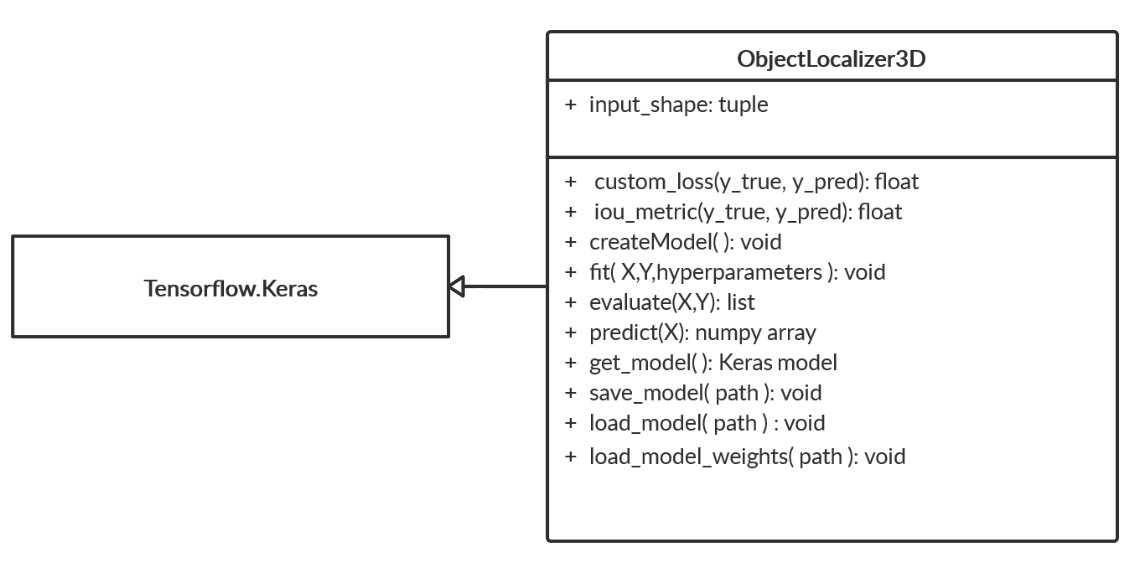
\includegraphics[width=14.2cm]{Abb/ULM_class_objectLocalizer.PNG}
  \caption{UML Diagramm der Klasse ObjectLocalizer3D (abgeleitet von \textit{Keras Functional API})}
  \label{UML_localizer}
\end{figure} 


  